\section{PROCEDIMENTOS METODOLÓGICOS}

Os procedimentos metodológicos definem as principais atividades realizadas para o desenvolvimento deste trabalho, incluindo as pesquisas, o desenvolvimento e avaliação do \textit{software}. Nas seções a seguir, descrevemos essas etapas.

\subsection{Definição do Processo}
Processos de \textit{software} são utilizados pelos engenheiros de \textit{software} para controlar e coordenar projetos de desenvolvimento de \textit{softwares} reais \cite{talma2006desenvolvimento}. \citeonline{padua2003engenharia} descreve um processo como um conjunto de passos parcialmente  ordenados, constituídos por atividades, métodos, práticas e transformações, usado para atingir uma meta. Desta forma, um modelo de processo de \textit{software} é uma descrição simplificada de um processo, sendo também uma representação abstrata do mesmo para explicar as diferentes abordagens de desenvolvimento \cite{sommerville2003engenharia}.

Processos de software são complexos e dependem do julgamento humano como em qualquer processo intelectual, sendo assim, não existe um processo de software ideal, todos são desenvolvidos de maneiras diferentes por cada organização \cite{sommerville2003engenharia}.

O processo de \textit{software} utilizado para desenvolver o sistema foi baseado no modelo cascata, também chamado de ciclo de vida clássico, proposto por Royce em 1970. Neste modelo, as fases são sistematicamente seguidas de maneira sequencial \cite{pressman2006engenharia}. O modelo inicia com a fase de especificação de requisitos, passando pelo planejamento, modelagem, construção e implantação, finalizando na manutenção progressiva do software, como apresentamos na \autoref{figura_ciclo_cascata}.

As vantagens desse modelo se devem ao fato de que só se avança para a tarefa seguinte quando o cliente valida e aceita os produtos finais da tarefa atual, facilitando assim a compreensão adquirida ao longo do projeto, além de facilitar o processo de criação da documentação para o sistema \cite{pressman2006engenharia}. Já as principais desvantagens segundo \citeonline{pressman2006engenharia}, se devem ao fato de que os projetos reais raramente seguem o fluxo sequencial ao qual o modelo propõe; o mesmo afirma ainda que este modelo exige que todos os requisitos sejam estabelecidos na fase inicial, fato que geralmente é difícil tanto para o cliente quanto para o desenvolvedor, já que os requisitos mudam constantemente. Outro grande problema com esse modelo é que o cliente só recebe uma versão executável do sistema no final de todo o processo de desenvolvimento, o que não agrada a muitos clientes.

Levando em consideração as vantagens e desvantagens antes citadas, esse modelo foi escolhido como base para o processo por facilitar o desenvolvimento de uma documentação mais detalhada e principalmente pela equipe de desenvolvimento ser formada por uma única pessoa, o autor deste trabalho, impossibilitando assim, uma divisão de tarefas durante o desenvolvimento, característico de metodologias ágeis \footnote{Metodologias de desenvolvimento de software que tem enfoco nas pessoas e não em processos ou algoritmos, além de uma preocupação menor em documentação e maior em implementação \cite{michel2004metodologias}.}.

\begin{figure}[H]
\centering
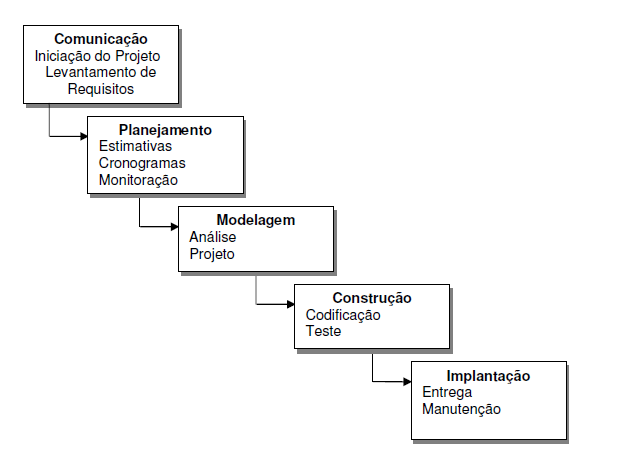
\includegraphics[width=10cm]{figuras/figura_ciclo_cascata}
\caption{Modelo Cascata (fonte: \citeonline{pressman2006engenharia}  )}
\label{figura_ciclo_cascata}
\end{figure}

O processo desenvolvido pode ser encontrado no \autoref{apendice_processo}.

\subsection{Levantamento e Análise de Requisitos}


O Levantamento de Requisitos é a fase do desenvolvimento de um software onde o analista verifica junto ao usuário, quais as necessidades, condições e princípios que o \textit{software} deverá atender \cite{matuda2013mapas}. Essa fase possibilitou conhecer e estudar as necessidades do cliente, assim como as restrições que o software estará sujeito.

Para realizar a coleta dos requisitos, optamos por utilizar entrevistas com o cliente. Nessas entrevistas, que se caracterizarão como semi-estruturadas, já que foram guiadas por um roteiro previamente elaborado, composto por questões abertas \cite{belei2008uso}, foi possível obter os requisitos do sistema, assim como o público-alvo a quem o sistema atenderá. Essa técnica foi utilizada porque permitia uma organização flexível e ampliação dos questionamentos à medida que as informações foram sendo fornecidas pelo cliente \cite{fujisawa2000utilizaccao}.

Para uma melhor compreensão do público-alvo, foram criadas Personas 
\cite{pruitt2003personas}, personagens fictícios usados para caracterizar os papéis dos diferentes usuários do sistema \cite{guerra2010colaboraccao}, cada persona criada possuía um nome, hábitos, histórias pessoais, motivações, objetivos, entre outras (ver \autoref{apendice_personas}). A escolha dessa técnica deu-se pelo fato de que ela permitia ao desenvolvedor saber mais precisamente para quem ele deveria construir o sistema, além de permitir uma distinção maior do público-alvo e dessa forma, aprofundar-se nos interesses individuais de cada um.

Após o levantamento dos requisitos, foi realizado uma análise dos mesmos. Nessa análise, os requisitos foram agrupados em categorias. As categorias utilizadas são descritas por \citeonline{sommerville2003engenharia} como:
\begin{alineascomponto}
    \item Requisitos Funcionais: especificam ações que um sistema deve ser
capaz de executar, sem levar em consideração restrições físicas. Os requisitos
funcionais especificam, portanto, o comportamento de entrada e saída de um
sistema.
    \item Requisitos Não Funcionais: descrevem apenas atributos do sistema ou
atributos do ambiente do sistema, como segurança, desempenho, usabilidade e
confiabilidade.
    \item Requisitos de Domínio: são os requisitos do domínio da aplicação do sistema e que refletem características desse domínio.
\end{alineascomponto}

Após esse agrupamento, os requisitos funcionais foram representados em Casos de Uso \cite{jacobson92engenharia}, um caso de uso identifica os agentes envolvidos em uma interação e especifica o tipo de interação, utilizando anotações sugeridas pela Unified Modeling Language (UML) 
\citeonline{sommerville2003engenharia}. Em seguida, foi realizada a documentação dos requisitos (ver \autoref{apendice_requisitos}).

Na etapa final dessa fase, ocorreu a Validação dos Requisitos junto ao cliente.  A Validação dos Requisitos é definida como o processo que certifica que o modelo de requisitos gerado  esteja  consistente  com  as  necessidades  e  intenções  de  clientes  e usuários \cite{rilston2003metodologia}. Esta etapa permitiu que os requisitos coletados e documentados estejam de acordo com o que o cliente solicitou.

\subsection{Projeto do Sistema}

O Projeto de Software é à atividade de engenharia cujo foco é definir ``como'' os requisitos estabelecidos do projeto devem ser implementados no software \cite{pressman2006engenharia}. O objetivo da  atividade de projetar é gerar um modelo ou representação que apresente solidez, comodidade e deleite \cite{pressman2006engenharia}. 

Nesta fase, definimos como será aplicado o conhecimento obtido na pesquisa bibliográfica para se desenvolver o sistema. Para isto, definimos a arquitetura de software e as ferramentas que serão utilizadas durante o desenvolvimento do sistema. Nas seções a seguir, descrevemos um pouco sob cada um.

\subsubsection{Arquitetura}
Por arquitetura de software, entende-se a estrutura ou a organização de componentes de módulos, a maneira através da qual esses componentes interagem e a estrutura de dados que será usada pelos componentes \cite{pressman2006engenharia}.

A arquitetura utilizada baseia-se na arquitetura Cliente-Servidor\cite{david2013everything}, onde o processamento é dividido em processos distintos. Um processo é responsável pela manutenção da informação (servidor) e os outros são responsáveis pela captação de dados (clientes). Nessa arquitetura, os clientes enviam pedidos para o servidor, e este por sua vez processa estes dados e envia as respostas dos pedidos aos clientes.

Este modelo de arquitetura facilitará na manutenção do sistema, tendo em vista que toda atualização só necessitará ser realizada no servidor e automaticamente a mesma se propagará para todos os clientes. Com todos os recursos centralizados no servidor, podemos também ter um maior ganho com segurança, já que podemos centralizar os nossos esforços para manter a segurança das informações em apenas um único ponto, além de possibilitar que apenas cliente credenciados possam acessar e/ou alterar essas informações. Uma das outras grandes vantagens que temos  ao utilizar esse modelo, é que a medida que a quantidade de clientes aumente, será possível suprir esses clientes sem necessitar realizar nenhuma modificação essencial.

Para uma visualização mais detalhada da arquitetura de software definida, visitar o  \autoref{apendice_arquitetura}.

\subsubsection{Ferramentas}

 A análise do sistema foi feita com o auxílio da ferramenta de criação de diagramas Astah \cite{astah2016}, a implementação com a linguagem Python \cite{vanrossum2010python}, com o sistema de gerenciamento de banco de dados PostgresSQl \cite{momjian2001postgresql} e a camada de aplicação através da utilização do framework Django \cite{django2016}. Assim como a utilização do módulo Rosseta \cite{rosetta2016} para permitir a internacionalização do sistema.
 
A seguir a lista das ferramentas e das tecnologias utilizadas para o desenvolvimento do projeto:

\begin{alineas}
	\item Astah: Para a modelagem baseada em UML (Unified Modeling Language) do sistema.
	\item Python: Linguagem de programação para implementação do sistema.
    \item Django: Framework web responsável pela camada de aplicação.
    \item Rosetta: Aplicação desenvolvida em Django que facilitará a tradução do projeto para diversas línguas.  
    \item PostgreSQL: Como banco de dados para armazenamento e consulta de informações.
    \item Metro UI Css: Framework que faz uso de HTML, Cascading Stype Sheet (CSS) e Javascript para criação do front-end do sistema.
    \item MathJax: É uma engine\footnote{Uma biblioteca ou pacote de funcionalidades que são utilizadas para facilitar o desenvolvimento de alguma tecnologia.} de código aberto desenvolvido em javascript na forma de um plugin para incluir equações matemáticas em todos os navegadores, esse plugin aceita expressões em  MathML e Latex.

\end{alineas}

Essas ferramentas foram selecionadas por se tratarem, algumas, de ferramentas Open Source, ou seja, que seu código-fonte fonte pode ser alterado para diferentes fins, possibilitando assim que qualquer um consulte, examine ou as modifique,e outras por serem ferramentas que possibilitam um rápido desenvolvimento.

No final dessa fase, foi gerado o Plano de Projeto (ver \autoref{apendice_projeto}), esse documento guiar\'a os desenvolvedores durante 
todo o processo de desenvolvimento.

\subsection{Implementação do Sistema}

A implementação envolve as atividades de codificação, compilação e integração. A codificação visa traduzir o design num programa, utilizando linguagens e  ferramentas adequadas. A codificação deve refletir a estrutura e o comportamento descrito no projeto. Os componentes arquiteturais devem ser codificados de forma independente e depois integrados \cite{aguiar2012requisitos}.

\subsection{Verificação e Validação}
Essa fase destina-se a mostrar que o sistema está de acordo com a especificação 
e que ele atende às expectativas de clientes e usuários. Al\'em de assegurar 
que o  programa está fazendo aquilo que foi definido na sua especificação e não 
possui  erros  de  execução \cite{aguiar2012requisitos}. 

Durante essa fase, ser\~ao realizados Testes de Unidade e Integra\c{c}\~ao em 
cada modulo do sistema, assim como Testes de Sistema no sistema como um todo.

\citeonline{aniche2014teste} define essas categorias de Testes de Software como:

\begin{alineascomponto}
	\item Teste de Unidade é aquele que testa uma única unidade do sistema. 
Ele a testa de maneira isolada, geralmente simulando as prováveis dependências 
que aquela unidade tem. Em sistemas orientados a objetos, é comum que a unidade 
seja uma classe. Ou seja, quando queremos escrever testes de unidade para a 
classe Pedido, essa bateria de testes testará o funcionamento da classe Pedido, 
isolada, sem interações com outras classes.

	\item  Teste de Integração é aquele que testa a integração entre duas 
partes do seu sistema. Os testes que você escreve para a sua classe PedidoDao, 
por exemplo, onde seu teste vai até o banco de dados, é um teste de integração. 
Afinal, você está testando a integração do seu sistema com o sistema externo, 
que é o banco de dados. Testes que garantem que suas classes comunicam-se bem 
com serviços web, escrevem arquivos texto, ou mesmo mandam mensagens via socket 
são considerados testes de integração.

	\item Teste de Sistema garante que o sistema funciona como um todo. Este 
nível de teste está interessado se o sistema funciona como um todo, com todas as 
unidades trabalhando juntas. Ele é comumente chamado de teste de caixa preta, já 
que o sistema é testado “com tudo ligado”: banco de dados, serviços web, batch 
jobs, e etc. 
\end{alineascomponto}

\subsection{Definição dos Conteúdo para o Sistema}

Após o sistema está verificado e validado, ele terá que possui conteúdos para ser utilizado pelo usuário final durante a fase de aplicação. 

Sendo que a aplicação da primeira versão do sistema está planejada para ocorrer com uma turma de matemática da Universidade Federal do Ceará - Campus Quixadá, decidimos optar por deixar os monitores\footnote{É o aluno de graduação concursado para exercer, juntamente com o professor, atividades técnico-didáticas condizentes com o seu grau de conhecimento junto à determinada disciplina, já por ele cursada.} da disciplina desenvolver o conteúdo que será utilizado no sistema durante essa fase. 

Os monitores passaram por um treinamento, onde aprenderam a utilizar o sistema para assim, adicionar os conteúdos desenvolvidos.

\subsection{Aplicação da Solução na Universidade Federal do Ceará - Campus Quixadá}

Essa fase tem por objetivo, permitir que sejam coletados dados para verificar o impacto da ferramenta com usuários reais. Para isso, aplicaremos o sistema em metade da turma de uma disciplina de Matemática Básica da UFC - Campus Quixadá, sendo que a outra metade não utilizará o sistema.

Nosso objetivo nessa fase, é verificar a evolução no aprendizado dos alunos dessa turma, sejam os que utilizaram o sistema como também os que não utilizaram. Para tentar verificar qualquer tipo de mudança que a ferramenta possa ter gerado nos alunos que a utilizaram.  

\subsection{Cronograma de Execução}
\begin{table}[H]
\centering
\caption{Cronograma de Execução}
\label{cronograma}

\resizebox{\textwidth}{!}{
\begin{tabular}{|l|c|c|c|c|c|c|c|c|c|c|c|c|c|c|c|}
\hline
\multicolumn{1}{|c|}{\multirow{2}{*}{ATIVIDADES}} & \multicolumn{6}{c|}{2015} & \multicolumn{9}{c|}{2016} \\ \cline{2-16} 
\multicolumn{1}{|c|}{} & Jan & Fev & Mar & Abr & Mai & Jun - Dez & \multicolumn{1}{l|}{Jan - Mar} & \multicolumn{1}{l|}{Abr} & \multicolumn{1}{l|}{Mai} & \multicolumn{1}{l|}{Jun} & \multicolumn{1}{l|}{Jul} & \multicolumn{1}{l|}{Ago} & \multicolumn{1}{l|}{Set} & \multicolumn{1}{l|}{Out} & \multicolumn{1}{l|}{Nov} \\ \hline
Definição do Processo & x &  &  &  &  &  &  &  &  &  &  &  &  &  &  \\ \hline
Levantamento e Análise dos Requisitos & x & x & x &  &  &  &  &  &  &  &  &  &  &  &  \\ \hline
Projeto do Sistema &  &  &  & x & x &  &  &  &  &  &  &  &  &  &  \\ \hline
Implementação do Sistema &  &  &  &  &  & x & x & x & x & x &  &  &  &  &  \\ \hline
Verificação e Validação &  &  &  &  &  &  &  &  &  &  & x &  &  &  &  \\ \hline
Desenvolver o conteúdo para o sistema &  &  &  &  &  &  &  & x & x & x & x & x &  &  &  \\ \hline
Aplicação na UFC - Campus Quixadá &  &  &  &  &  &  &  &  &  &  &  & x & x & x &  \\ \hline
Definição do Projeto de Pesquisa &  &  &  &  &  &  &  & x &  &  &  &  &  &  &  \\ \hline
Defesa do Projeto de Pesquisa &  &  &  &  &  &  &  &  &  & x &  &  &  &  &  \\ \hline
Ajustes Solicitados &  &  &  &  &  &  &  &  &  &  & x &  &  &  &  \\ \hline
Análise dos Resultados Obtidos na Aplicação. &  &  &  &  &  &  &  &  &  &  &  &  &  &  & x \\ \hline
Defesa do Trabalho Final &  &  &  &  &  &  &  &  &  &  &  &  &  &  & x \\ \hline
\end{tabular}}
\fnote{Fonte: Elaborado pelo autor}
\end{table}
